\begin{figure}[ht]
	\centering
	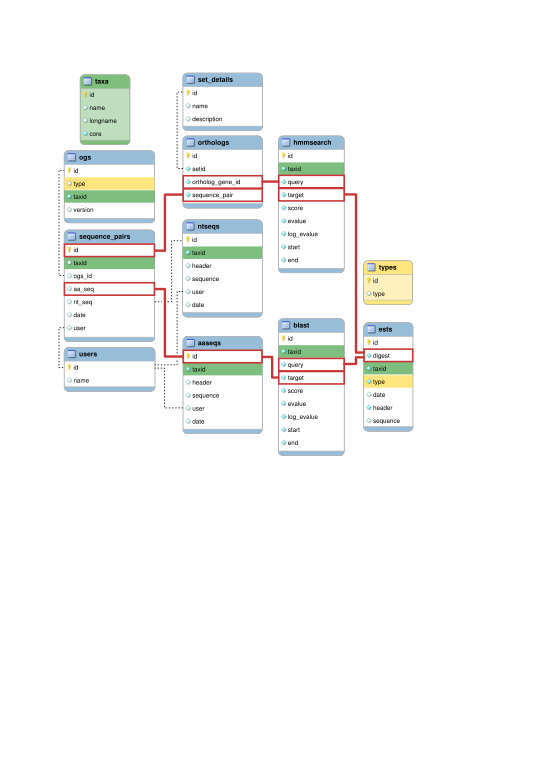
\includegraphics[width=\textwidth]{img/dbstructure.pdf}
	\caption[Complete \pname database structure]{
		\pname database structure. Each rounded rectangle represents a table with
		named columns. Note the circular path (red) that can be drawn across the
		tables and that is used in special \code{JOIN} queries in order to construct
		a graph of orthologous relationships. Green table columns are referenced to
		the ``taxa'' table, and yellow table columns are referenced to the ``types''
		table. Dotted lines are secondary references.
	}
	\label{fig:dbstructure}
\end{figure}


